% Slide 6: [Rubric Mục 5 - 10%] Storyboard - Bảng Phân Cảnh Trực Quan
\begin{frame}{Mục 5: Storyboard -- Bảng Phân Cảnh Trực Quan}
  \framesubtitle{\color{PetcareSecondary}\textbf{[Rubric: 10\%] Câu chuyện trải nghiệm hấp dẫn $\bullet$ 6 Khung tranh trực quan $\bullet$ Chú thích chi tiết}}

  \begin{columns}[T]
    % Cột trái: Hình ảnh Storyboard thực tế từ báo cáo
    \begin{column}{0.48\textwidth}
      \centering
      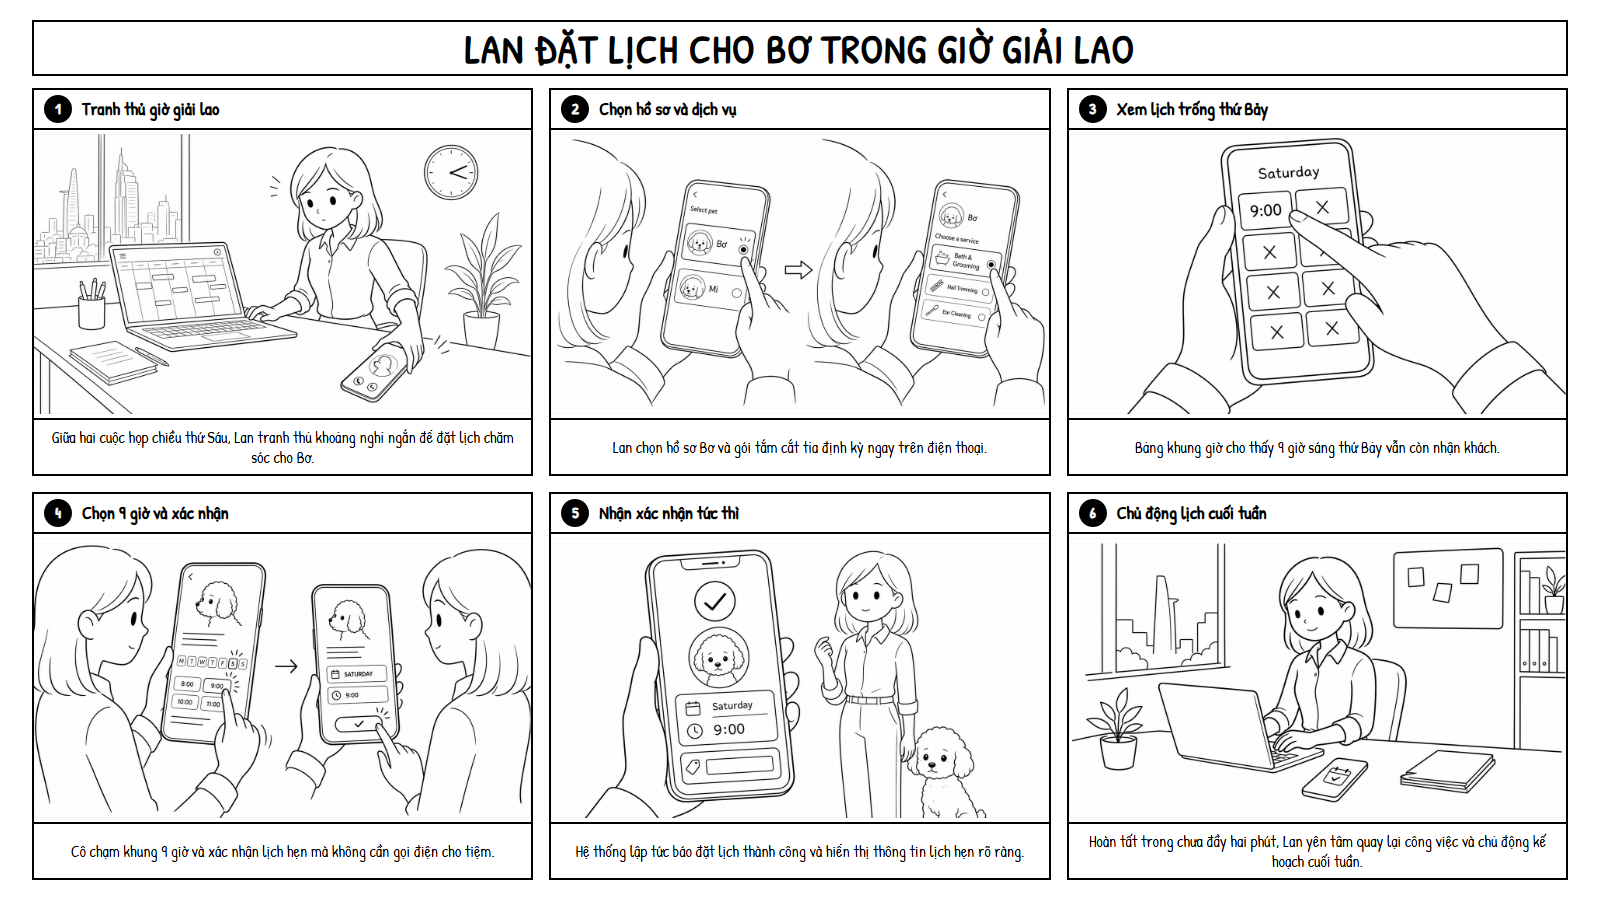
\includegraphics[width=\linewidth, height=4.3cm, keepaspectratio]{img/storyboard-p1-g1.png}\\[1mm]
      {\tiny \color{PetcareDark}\textbf{Minh họa:} Bảng phân cảnh 6 khung tranh Goal 1 của Persona 1 (Chị Lan)}
    \end{column}

    % Cột phải: 6 Khung cảnh câu chuyện & Chú thích chi tiết
    \begin{column}{0.50\textwidth}
      \begin{block}{\footnotesize \textbf{Diễn biến câu chuyện 6 khung hình (Story Flow)}}
        \begin{enumerate}
          \setlength\itemsep{0.5mm}
          \tiny
          \item \textbf{Khung 1 -- Nhu cầu bận rộn:} Chị Lan tại văn phòng mở app chọn dịch vụ tắm thảo dược và giờ trống cho Poodle Bơ.
          \item \textbf{Khung 2 -- Xác nhận tức thì:} Hệ thống cấp ngay mã QR và tự nạp cảnh báo đỏ dị ứng xà phòng mà không cần chờ duyệt.
          \item \textbf{Khung 3 -- Bàn giao an toàn tại tiệm:} Nhân viên quét QR, cam kết dùng đúng sữa tắm hữu cơ qua biên bản 2 lớp.
          \item \textbf{Khung 4 -- Theo dõi từ xa tại công ty:} Lan an tâm họp hành khi thanh tiến trình cập nhật mốc \textit{Đang chăm sóc}.
          \item \textbf{Khung 5 -- Đón bé đúng hẹn:} Nhận thông báo mời đón, Lan đến tiệm nhận Bơ khỏe mạnh, không bị kích ứng da.
          \item \textbf{Khung 6 -- Lưu trữ \& Đặt lại:} Lan mở nhật ký xem lại hóa đơn và bấm nút Rebook hẹn lịch cho 2 tuần sau.
        \end{enumerate}
      \end{block}

      \vspace{-1mm}
      \begin{exampleblock}{\scriptsize \textbf{Chuẩn mực nghệ thuật HCI}}
        \tiny
        Phong cách \textbf{Expressive UI Storytelling}: Thể hiện trọn vẹn sự chuyển biến cảm xúc từ \textit{Bất an, căng thẳng} sang \textit{Nhẹ nhõm, an tâm tuyệt đối}.
      \end{exampleblock}
    \end{column}
  \end{columns}
\end{frame}
